\section{Lab: Copy-on-Write Fork for xv6}
\subsection{实验目的}

本实验旨在促进了解写时复制(Copy-On-Write,COW)机制,同时增进对fork函数分配内存机制的理解。在 xv6 操作系统内核中实现COW机制。通过实现 COW 机制,可以在fork 系统调用时避免直接复制父进程的所有内存页,从而提高内存使用效率。当子进程尝试写入共享页面时,再复制相应的页面。

\subsection{实验步骤}

\begin{enumerate}
    \item 首先,修改riscv.h文件,添加一个页表标志位PTE\_COW,用于记录页表是否处于COW状态。
          \begin{lstlisting}[language=c,title=对riscv.h文件的修改]
    #define PTE_V (1L << 0) // valid
    #define PTE_R (1L << 1)
    #define PTE_W (1L << 2)
    #define PTE_X (1L << 3)
    #define PTE_U (1L << 4) // 1 -> user can access
    #define PTE_COW (1L << 8) // 1 -> cow page
    \end{lstlisting}
    \item 在kalloc.c文件中添加一个数组int reference[PHYSTOP / PGSIZE]记录页表引用数,并设置一个锁确保对数组的安全操作。
          \begin{lstlisting}[language=c,title=添加记录引用数的数组和锁]
    int reference[PHYSTOP / PGSIZE];
    struct spinlock refcountlock;
    \end{lstlisting}
    \item 修改kalloc函数和kfree函数,实现对reference数组的初始化和页面释放。
          \begin{lstlisting}[language=c,title=对kalloc函数的修改]
    void *kalloc(void)
    {
        struct run *r;

        acquire(&kmem.lock);
        r = kmem.freelist;
        
        // 如果有空闲页面,分配给请求者
        if (r)
        {
            kmem.freelist = r->next;
            // 添加部分
            acquire(&refcountlock);
            reference[((uint64)r) / PGSIZE] = 1;
            release(&refcountlock);
        }
        release(&kmem.lock);

        if (r)
            memset((char *)r, 5, PGSIZE); // fill with junk
        return (void *)r;
    }
    \end{lstlisting}
          \begin{lstlisting}[language=c,title=对kfree函数的修改]
    void kfree(void *pa)
    {
        struct run *r;
        
        if (((uint64)pa % PGSIZE) != 0 
        || (char *)pa < end 
        || (uint64)pa >= PHYSTOP)
            panic("kfree");

        // 添加部分,减少引用计数
        acquire(&refcountlock);
        reference[((uint64)pa) / PGSIZE]--;
        release(&refcountlock);
        if (reference[((uint64)pa) / PGSIZE] > 0)
            return;

        // Fill with junk to catch dangling refs.
        memset(pa, 1, PGSIZE);

        r = (struct run *)pa;

        acquire(&kmem.lock);
        r->next = kmem.freelist;
        kmem.freelist = r;
        release(&kmem.lock);
    } 
    \end{lstlisting}
    \item 修改trap.c文件,添加一个cowhandler函数并修改usertrap函数,当发生缺页异常,为进程复制一个新物理页面。
          \begin{lstlisting}[language=c,title=cowhandler函数的实现]
    int cowhandler(pagetable_t pagetable, uint64 va)
    {
        char *mem;
    
        // 检查虚拟地址是否超过最大有效地址
        if (va >= MAXVA)
            return -1;
        // 获取页表条目(PTE)
        pte_t *pte = walk(pagetable, va, 0);
        if (pte == 0)
            return -1;   
        // 检查PTE是否有效、用户模式、COW标志
        if ((*pte & PTE_V) == 0 || (*pte & PTE_U) == 0 || (*pte & PTE_COW) == 0)
            return -1;
        // 分配一个新的物理页面
        if ((mem = kalloc()) == 0)
            return -1; 
        // 获取原物理地址
        uint64 pa = PTE2PA(*pte);
        // 将原物理页面内容复制到新页面
        memmove((char *)mem, (char *)pa, PGSIZE);
        // 释放原物理页面
        kfree((void *)pa);
        // 获取PTE的标志位
        uint flags = PTE_FLAGS(*pte);
        // 更新PTE指向新物理页面,并设置为可写
        *pte = (PA2PTE(mem) | flags | PTE_W);
        // 清除COW标志
        *pte &= ~PTE_COW;
    
        return 0;
    }            
    \end{lstlisting}
          \begin{lstlisting}[language=c,title=对usertrap函数的修改]
    void usertrap(void)
    {
        ...

        // 检查陷阱原因
        if (r_scause() == 8)
        {
            ...
        }
        else if (r_scause() == 15)
        {
            // 处理Copy-On-Write(COW)错误
            uint64 va = r_stval();
            if (va >= p->sz)
                p->killed = 1;
            int ret = cowhandler(p->pagetable, va);
            if (ret != 0)
                ->killed = 1;
        }
        else if ((which_dev = devintr()) != 0)
        {
            // 设备中断
            // ok
        }
        else
        {
            ...
        }

        ...
        
        usertrapret();
    }
    \end{lstlisting}
    \item 在vm.c文件中修改copyout函数,添加COW页面的处理逻辑。
          \begin{lstlisting}[language=c,title=对copyout函数的修改]
    int copyout(pagetable_t pagetable, uint64 dstva, char *src, uint64 len)
    {
        uint64 n, va0, pa0;

        while (len > 0)
        {
            ...

            // 如果是Copy-On-Write页面,处理COW逻辑
            if (checkcowpage(va0, pte, p))
            {
                char *mem;

                // 分配一个新的物理页面
                if ((mem = kalloc()) == 0)
                {
                    p->killed = 1;
                }
                else
                {
                    // 将原页面的数据复制到新页面
                    memmove(mem, (char *)pa0, PGSIZE);

                    // 获取页表条目的标志位
                    uint flags = PTE_FLAGS(*pte);

                    // 解除原页面映射
                    uvmunmap(pagetable, va0, 1, 1);

                    // 更新页表条目,指向新页面并设置为可写
                    *pte = (PA2PTE(mem) | flags | PTE_W);

                    // 清除COW标志
                    *pte &= ~PTE_COW;

                    // 更新物理地址
                    pa0 = (uint64)mem;
                }
            }

            ...
        }

        return 0;
    }
    \end{lstlisting}
\end{enumerate}

\subsection{评测结果}
利用grade-lab-cow脚本评测,得到结果如图\ref{fig:cow}。
\begin{figure}[h]
    \centering
    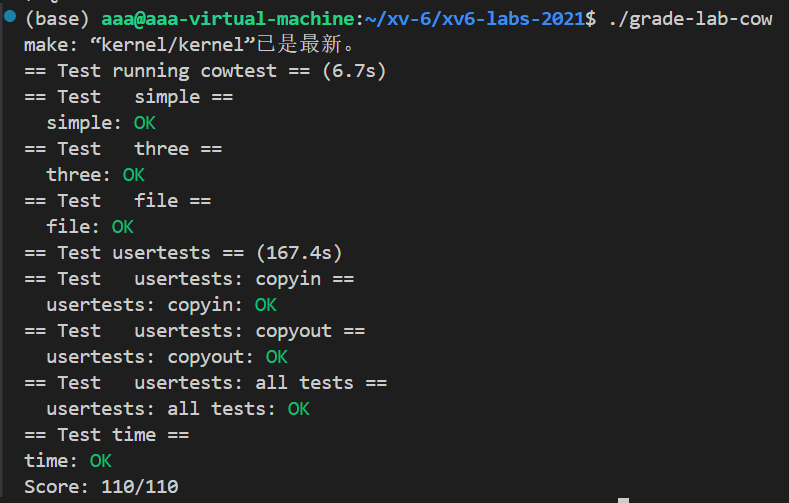
\includegraphics[width=\linewidth]{pics/cow评测结果.png}
    \caption{评测结果}
    \label{fig:cow}
\end{figure}

\subsection{实验小结}
本次实验通过在 xv6 操作系统内核中实现写时复制(Copy-On-Write,COW)机制,加深了我对内存管理和进程创建的理解。在传统的fork系统调用中,父进程的所有内存页都会被直接复制给子进程,而COW机制通过延迟实际的内存复制操作,提高了内存使用效率。

通过实验,我不仅掌握了COW机制的基本原理,还增强了对操作系统内存管理和进程管理的理解,提升了在操作系统内核中进行实际编程和调试的能力。这些技能对于理解和开发高效的操作系统具有重要意义。
